\subsection{Historical Evolution of Crowd Simulation}

Over the past three decades, crowd simulation research has evolved from macroscopic flow-based approximations to sophisticated multi-agent systems capable of real-time interaction at massive scales. Early approaches emphasized reproducing emergent collective phenomena, while later developments focused on predictive collision avoidance, behavioral realism, and numerical stability under high-density conditions. This progression reflects a gradual shift from aggregate modeling toward constraint-based and adaptive frameworks designed to balance realism with computational scalability.

\subsubsection{Macroscopic and Hybrid}
When it comes to dealing with large-scale crowd simulation, handling collision avoidance is a major challenge. In Continuum Crowds \cite{treuille2006continuum}, macroscopic approach based on continuum dynamics is introduced, where a dynamic potential field integrates global navigation and obstacle avoidance into a single framework. By treating the crowd as a continuous density field rather than individual particles, the model naturally produces emergent phenomena like lane formation and vortices. While computationally efficient, the continuum approach tends to too simplify the crowd, failing to account for individual behaviors and interactions, which can lead to unrealistic results in scenarios where individual decision-making is crucial.

Bridging the gap between microscopic and macroscopic approaches, Narain et al. \cite{narain2009aggregate} introduced Aggregate Dynamics for Dense Crowd Simulation with a dual representation that models the crowd simultaneously as discrete agents and as a continuous system, governed by their unilateral incompressibility constraint (UIC). This allows the simulation to capture the emergent phenomena of large crowds while maintaining individual agent behaviors, providing realistic simulation even with extremely large dense crowds of up to 100,000 agents. However, the approach with UIC simplifies behavioral modeling by optimizing primarily for progress toward desired destinations, which may not fully capture the complex behavioral features observed in real human crowds.

\subsubsection{Microscopic and Adaptive}

Collision avoidance is a critical aspect in crowd simulation. Many early models relied on reactive force-based approaches where agents would respond to the environment and other agents when they were within a certain proximity. However, Karamouzas et al. \cite{Karamouzas2009Predictive} demonstrated that humans anticipate collisions and adjust their paths long in advance. By using a velocity-based approach where agents predict the time to contact, they achieved smoother, more energy-efficient trajectories that avoid the "oscillations" common in earlier reactive models.

\begin{figure}[ht]
    \centering
    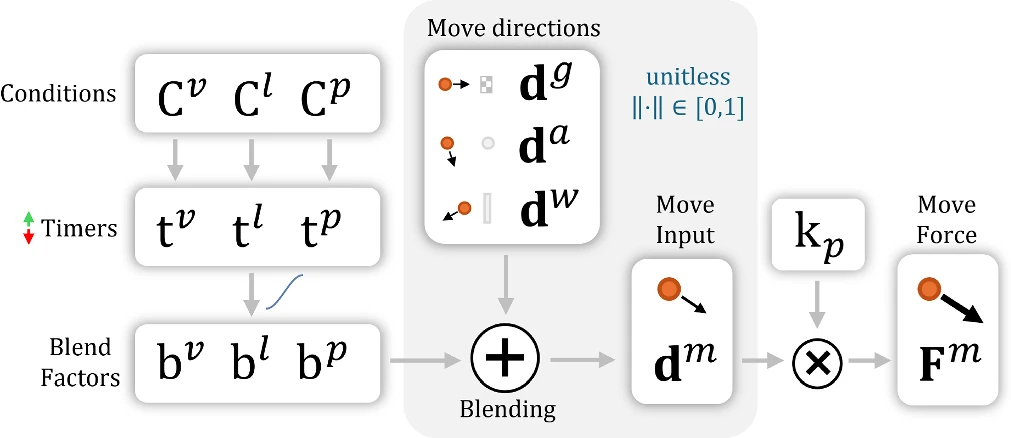
\includegraphics[width=0.5\textwidth]{img/BlendFactor.png}
    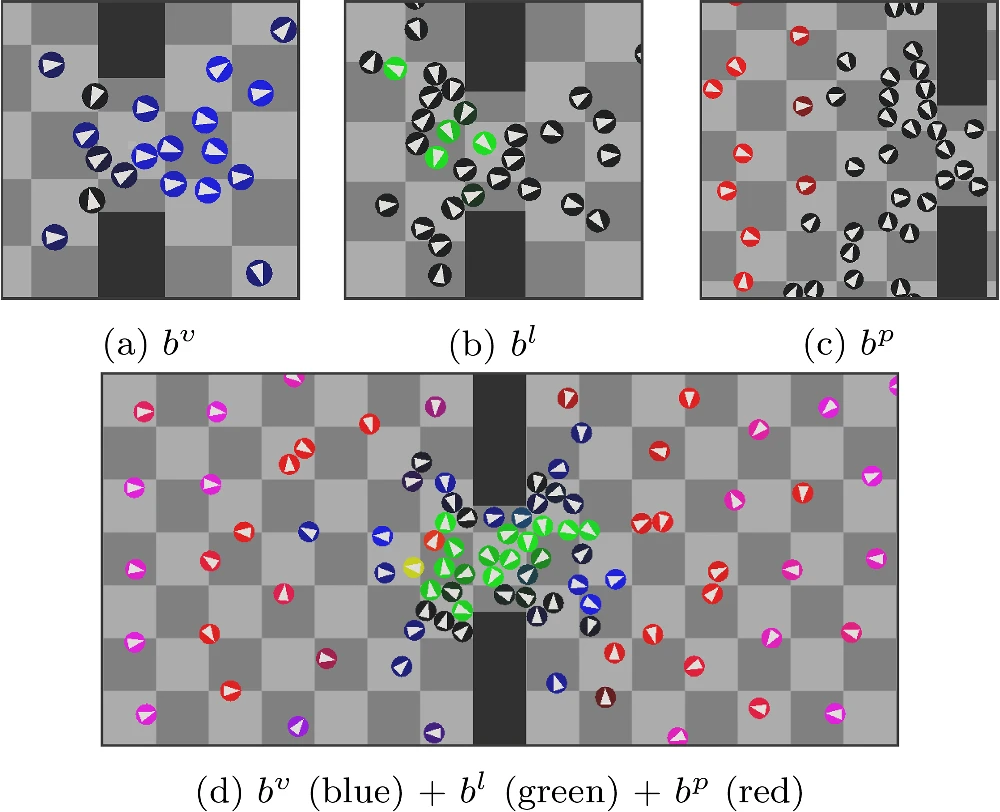
\includegraphics[width=0.5\textwidth]{img/BlendFactor2.png}
    \caption{Adaptive movement behavior in crowd simulation showing context-dependent blending between goal-oriented and avoidance-centric behaviors.}
    \label{fig:adaptive_behavior}
\end{figure}

The recent work by Ruprecht et al. \cite{Ruprecht2024Adaptive}, Adaptive Movement Behavior for Real-Time Crowd Simulation, introduces situational awareness. While earlier models focused on the physics of avoidance, this paper addresses the synthesis of global path planning and local collision avoidance through context-dependent blending. By employing direction-aware neighbor sets and adaptively shifting between goal-oriented and avoidance-centric behaviors, the model allows agents to navigate complex environments with a degree of social and environmental context previously missing from force-based simulations \ref{fig:adaptive_behavior}.


\subsection{Pathfinding in Multi-Agent Systems}

\subsubsection{Partial Refinement A*}

The A* algorithm is a widely used pathfinding method in game development and robotics. However, it can be computationally expensive in large, complex environments. Sturtevant and Buro \cite{Sturtevant2005PartialRefinement} introduced a partial refinement A* that uses map abstraction to create a simplified representation of the environment. This allows for faster pathfinding by first finding a path on the abstracted map and then refining it on the original map. While reducing computational overhead, this method may produce suboptimal paths due to the abstraction.

\begin{figure}[ht]
    \centering
    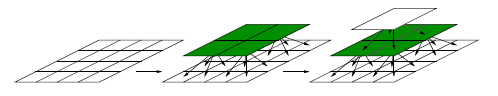
\includegraphics[width=0.8\textwidth]{img/PRA.png}
    \caption{Partial Refinement A* (PRA*) abstraction and refinement process. The original map is abstracted into a simplified representation, where pathfinding is first performed on the abstracted map. The resulting path is then refined on the original map to produce a more accurate route.}
    \label{fig:abstraction}
\end{figure}

\subsubsection{Direction Maps}
Cooperative pathfinding is one of the most significant topics in various fields, including robotics and computer games. The main challenge is from the complexity of the computation, which is often exponential in the number of agents. Direction maps, as proposed by Sturtevant and Jansen \cite{Sturtevant2008DirectionMap}, provide a way to guide agents to cooperate with other agents throughout movement and planning. 

\begin{figure}[ht]
    \centering
    \begin{subfigure}{0.5\textwidth}
        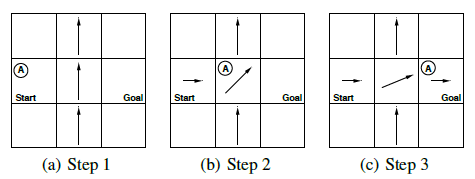
\includegraphics[width=\textwidth]{img/DV.png}
        \caption{Learning Direction Vector}
        \label{fig:direction_map_learning}
    \end{subfigure}
    \begin{subfigure}{0.3\textwidth}
        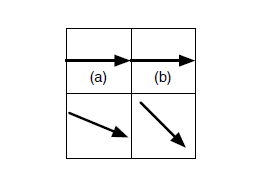
\includegraphics[width=\textwidth]{img/DM.png}
        \caption{Example of Planning with Direction Map}
        \label{fig:direction_map_example}
    \end{subfigure}
    \caption{Direction maps for cooperative pathfinding.}
    \label{fig:direction_map}
\end{figure}

By precomputing a direction map that indicates the encouraged direction for each agent to move based on the current state of the environment and other agents, this method allows for efficient pathfinding in multi-agent systems. Furthermore, in order to further reduce the computational cost, abstraction can be applied to the direction maps, where the environment is simplified into larger regions with uniform direction recommendations \cref{fig:direction_map_abstraction}. This allows for faster pathfinding while still providing effective guidance for agent cooperation.

\begin{figure}[ht]
    \centering
    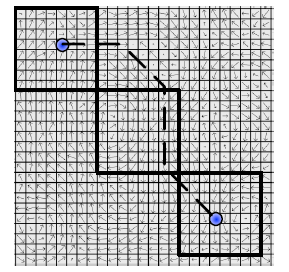
\includegraphics[width=0.25\textwidth]{img/abstraction.png}
    \caption{Abstraction can be applied in direction maps.}
    \label{fig:direction_map_abstraction}
\end{figure}







